%-----------------------------------------------------------------------------%
\chapter{\babEmpat}
\label{bab:4}
%-----------------------------------------------------------------------------%
Bab ini menjelaskan secara rinci tahapan yang penulis lakukan dalam melakukan
proses implementasi berdasarkan rancangan serta analisis yang telah dilakukan
pada bab sebelumnya. Proses yang penulis lakukan pada tahapan implementasi
antara lain: implementasi program, implementasi kebutuhan \textit{deployment}, dan
proses \textit{deployment}.

\section{Implementasi Aplikasi}
\label{sec:implementasiAplikasi}
Aplikasi yang telah dirancang pada \ref{sec:perancanganArsitektur} akan diimplementasikan. Bagian ini akan menjelaskan contoh dari kode yang merepresentasikan alur kerja aplikasi. Berkas sumber kode yang lengkap dapat dilihat pada lampiran \ref{appendix:hasilAplikasi}.

Implementasi program dimulai dengan melakukan inisiasi proyek pada Golang dengan melakukan \code{go mod init project-source}, dimana \code{project-source} merupakan lokasi sumber kode pada repositori GitHub milik GudangAda. Untuk memastikan repositori lebih teratur, penulis akan mengikuti konvensi dari \cite{golang-standards_2022} sebagai paduan untuk meletakkan berkas kode.

\subsection{Implementasi Bagian Utama Program}
\label{sec:maingo}
Kode utama pada aplikasi berisi inisiasi untuk membaca berkas konfigurasi, inisiasi \textit{router}, dan inisiasi \textit{HTTP listener}. Pada kode utama inilah \textit{server} berjalan untuk mendengarkan permintaan \textit{HTTP} dari \textit{host} dan \textit{port} yang telah diberikan.

\begin{lstlisting}[frame=single,language=Go,caption={Kode utama pada aplikasi yang dikembangkan},label={code:maingo}]
func main() {
	var rt routes.Route

	appConfigs, err := configs.InitAppConfigs()
	if err != nil {
		panic(err)
	}

	router := rt.Init(*appConfigs)

	var gracefulStop = make(chan os.Signal)
	signal.Notify(gracefulStop, syscall.SIGTERM)
	signal.Notify(gracefulStop, syscall.SIGINT)
	go func() {
		sig := <-gracefulStop
		fmt.Printf("caught sig: %+v", sig)
		fmt.Println("Wait for 2 second to finish processing")
		time.Sleep(2 * time.Second)
		os.Exit(0)
	}()

	headersOK := handlers.AllowedHeaders([]string{"X-Requested-With", "Content-Type", "NAME", "MODULE_NAME", "VERSION", "ON_FAILURE"})
	originsOK := handlers.AllowedOrigins([]string{"*"})
	methodsOK := handlers.AllowedMethods([]string{"GET", "POST", "OPTIONS", "DELETE", "PUT"})
	host := appConfigs.Server.Host
	port := strconv.Itoa(appConfigs.Server.Port)
	fmt.Println("Server served at port " + port)
	if err := http.ListenAndServe(host+":"+port, handlers.CORS(originsOK, headersOK, methodsOK)(router)); err != nil {
		log.Fatal("Unable to start service: " + err.Error())
	}
}
\end{lstlisting}

\subsection{Membaca Berkas Konfigurasi}
\label{sec:readConfig}
Nilai-nilai penting seperti \textit{credentials} ke \textit{Database}, pengaturan \textit{server}, \textit{password} ke Vault perlu didapatkan saat aplikasi pertama kali berjalan. Oleh karena itu, dibutuhkan sebuah fungsi yang dapat membaca \textit{file} konfigurasi saat aplikasi pertama kali dijalankan. Fungsi tersebut ada pada kode \ref{code:configInit}.

fungsi \code{InitAppConfig} pada kode \ref{code:configInit} bertugas untuk membaca konfigurasi dari \textit{environment} \textit{variable} atau dari \textit{file} konfigurasi. Data yang dibaca akan dimasukkan ke dalam sebuah variabel yang didefinisikan pada kode \ref{code:configStruct}. Variabel yang didapatkan akan dikembalikan ke fungsi utama pada kode \ref{code:maingo} untuk disebarkan lagi ke masing masing fungsi yang membutuhkannya.

\begin{lstlisting}[frame=single,language=Go,caption={\textit{Struct} yang berisi definisi variabel konfigurasi aplikasi},label={code:configStruct}]
type AppConfigs struct {
	Server     ServerConfig `yaml:"server"`
	Database   DBConfig     `yaml:"database"`
	Kubernetes AuthConfig   `yaml:"Kubernetes"`
	Vault      VaultConfig  `yaml:"vault"`
	ChartRepo  ChartRepo    `yaml:"chartRepo"`
}
\end{lstlisting}

\begin{lstlisting}[frame=single,language=Go,caption={Fungsi untuk membaca berkas konfigurasi},label={code:configInit}]
func InitAppConfigs() (*AppConfigs, error) {
	var appConfigs AppConfigs

	err := cleanenv.ReadEnv(&appConfigs)
	if err != nil {
		return nil, err
	}

	configFile := "config.yaml"
	if _, err := os.Stat(configFile); os.IsNotExist(err) {
		return &appConfigs, nil
	}

	err = cleanenv.ReadConfig(configFile, &appConfigs)
	if err != nil {
		return nil, err
	}

	return &appConfigs, nil
}
\end{lstlisting}

\subsection{Implementasi Koneksi ke Aplikasi Pihak Ketiga Pada Aplikasi}

Sesuai rancangan \ref{sec:aplikasiPihakKetiga}, aplikasi akan terkoneksi ke aplikasi pihak ketiga. Koneksi ke aplikasi pihak ketiga harus diinisiasikan terlebih dahulu sebelum dapat dipakai. Koneksi yang harus dibuat adalah koneksi ke \textit{Database}, Helm, Vault, dan Amazon Kinesis. Masing-masing inisiasi dilakukan dengan cara yang berbeda beda. Bagian ini akan menjelaskan cara aplikasi membuat koneksi ke masing masing aplikasi pihak ketiga.

\subsubsection{Inisiasi Koneksi ke \textit{Database}}
\label{sec:initDB}

Fungsi untuk mendapatkan koneksi ke \textit{database} yang didefinisikan pada kode \ref{code:databaseInit} diimplementasikan dengan \textit{design pattern singleton}. Inisiasi \textit{database} dilakukan dengan membuat koneksi ke \textit{database}, dan melakukan migrasi terhadap semua \textit{models} yang diperlukan.
\begin{lstlisting}[frame=single,language=Go,caption={Fungsi untuk inisiasi koneksi ke \textit{Database}},label={code:databaseInit}]
var database *gorm.DB

func GetDB(config configs.DBConfig) (*gorm.DB, error) {
	if database != nil {
		return database, nil
	}
	var err error
	dsn := fmt.Sprintf(
		"host=%s user=%s password=%s dbname=%s port=%d sslmode=allow TimeZone=UTC",
		config.Host,
		config.User,
		config.Password,
		config.Name,
		config.Port,
	)
	database, err = gorm.Open(postgres.Open(dsn), &gorm.Config{
		Logger: newLogger(),
	})
	if err != nil {
		return nil, err
	}

	err = database.AutoMigrate(&models.ChartRelease{})
	if err != nil {
		return nil, err
	}

	err = database.AutoMigrate(&models.Module{})
	if err != nil {
		return nil, err
	}

	err = database.AutoMigrate(&models.ModuleRelease{})
	if err != nil {
		return nil, err
	}

	err = database.AutoMigrate(&models.Kinesis{})
	if err != nil {
		return nil, err
	}

	return database, nil
}
\end{lstlisting}

\subsubsection{Inisiasi Koneksi ke Helm}
\label{sec:initHelm}

Khusus untuk koneksi ke Helm, tidak dapat diimplementasikan dengan \textit{singleton}. Hal ini terjadi karena pada kebutuhan K2, aplikasi harus dapat melakukan \textit{deployment} pada \textit{namespace} yang berbeda-beda. Namun, sebuah objek helm \textit{client} hanya dapat melakukan \textit{deployment} pada sebuah \textit{namespace} yang telah ditentukan sebelumnya. Oleh karena itu, akan dibuat N buah objek Helm \textit{Client} dimana N adalah jumlah \textit{namespace} yang dapat dikendalikan yang telah ditentukan pada inisiasi program melalui berkas konfigurasi.

Ada dua cara untuk mendapatkan akses ke helm. Cara pertama adalah melalui \textit{file} kubeconfig, cara ini biasanya dilakukan pada masa pengembangan di \textit{environment} lokal. Cara kedua adalah melalui \textit{serviceaccount} yang dihubungkan oleh Kubernetes, cara ini biasanya dilakukan untuk \textit{environment} \textit{production}.

\begin{lstlisting}[frame=single,language=Go,caption={Fungsi untuk inisiasi koneksi ke Helm},label={code:helmInit}]
func GenerateHelmClient(authConfig configs.AuthConfig) (map[string]helm.Client, error) {
	helmClient := map[string]helm.Client{}
	var config *rest.Config
	var err error

	switch authConfig.Method {
	case "kubeconfig":
		var kubeconfig *string
		if home := homedir.HomeDir(); home != "" {
			kubeconfig = flag.String("kubeconfig", filepath.Join(home, ".kube", "config"), "(optional) absolute path to the kubeconfig file")
		} else {
			kubeconfig = flag.String("kubeconfig", "", "absolute path to the kubeconfig file")
		}
		flag.Parse()

		config, err = clientcmd.BuildConfigFromFlags("", *kubeconfig)
		if err != nil {
			return nil, err
		}
	case "service-account":
		config, err = rest.InClusterConfig()
		if err != nil {
			panic(err.Error())
		}
	}

	for _, namespace := range authConfig.AvailableNamespace {
		opt := &helm.RestConfClientOptions{
			Options: &helm.Options{
				Namespace: namespace,
			},
			RestConfig: config,
		}

		helmClientTmp, err := helm.NewClientFromRestConf(opt)
		if err != nil {
			panic(err)
		}

		helmClient[namespace] = helmClientTmp
	}
	return helmClient, nil
}
\end{lstlisting}

\subsubsection{Inisiasi Koneksi ke Vault}
\label{sec:initVault}

Fungsi untuk mendapatkan koneksi ke Vault yang didefinisikan pada kode \ref{code:vaultInit} diimplementasikan dengan \textit{design pattern singleton}. Inisiasi \textit{database} dilakukan dengan membuat koneksi ke \textit{login} ke \textit{server} milik Vault. Ada dua cara untuk mendapatkan akses, yaitu melalui Kubernetes Service Account dan memasukkan \textit{password}. Penggunaan \textit{login} melalui Kubernetes Service Account biasanya dilakukan pada \textit{environment production}, sedangkan penggunaan \textit{login} melalui \textit{password} dilakukan untuk pengembangan aplikasi dalam \textit{environment local}.

\begin{lstlisting}[frame=single,language=Go,caption={Fungsi untuk inisiasi koneksi ke Vault},label={code:vaultInit}]
var vaultClient *api.Client

func GetVaultSecret(vaultConfig configs.VaultConfig) (*api.Client, error) {
	if vaultClient != nil {
		return vaultClient, nil
	}
	config := api.DefaultConfig()

	config.Address = vaultConfig.URL

	vaultClient, err := api.NewClient(config)
	if err != nil {
		return nil, err
	}

	var auth api.AuthMethod

	switch vaultConfig.AuthMethod {
	case "service-account":
		auth, err = Kubernetes.NewKubernetesAuth(
			vaultConfig.KubeMethod.RoleName,
			Kubernetes.WithMountPath(vaultConfig.KubeMethod.MountPath),
		)
		if err != nil {
			return nil, fmt.Errorf("unable to initialize Kubernetes auth method: %w", err)
		}
	case "userpass":
		auth, err = userpass.NewUserpassAuth(
			vaultConfig.UserPassMethod.Username,
			&userpass.Password{FromString: vaultConfig.UserPassMethod.Password},
		)
		if err != nil {
			return nil, fmt.Errorf("unable to initialize UserPass auth method: %w", err)
		}
	}

	authInfo, err := vaultClient.Auth().Login(context.TODO(), auth)
	if err != nil {
		return nil, fmt.Errorf("unable to log in with auth: %w", err)
	}
	if authInfo == nil {
		return nil, fmt.Errorf("no auth info was returned after login")
	}

	return vaultClient, nil
}
\end{lstlisting}

\subsubsection{Inisiasi Koneksi ke Amazon Kinesis}
\label{sec:initKinesis}

Fungsi untuk mendapatkan koneksi ke Amazon Kinesis yang didefinisikan pada kode \ref{code:kinesisInit} diimplementasikan dengan \textit{design pattern singleton}. Inisiasi objek dilakukan dengan membaca \textit{environment variable} atau dari \textit{serviceaccount}. Proses tersebut dilakukan secara otomatis oleh API yang disediakan oleh Amazon.

\begin{lstlisting}[frame=single,language=Go,caption={Fungsi untuk inisiasi Koneksi ke Amazon Kinesis},label={code:kinesisInit}]
var kinesisClient *kinesis.Client

func GetKinesisClient() (*kinesis.Client, error) {
	if kinesisClient != nil {
		return kinesisClient, nil
	}
	cfg, err := config.LoadDefaultConfig(context.TODO())
	if err != nil {
		return nil, err
	}
	kinesisClient = kinesis.NewFromConfig(cfg)
	return kinesisClient, nil
}
\end{lstlisting}

\subsection{Implementasi \textit{Routing} Aplikasi}
\label{sec:router}

Fungsi \textit{routing} pada aplikasi dimulai dengan melakukan inisiasi semua objek yang dibutuhkan yaitu Helm(fungsi pada kode \ref{code:helmInit}), Kinesis(fungsi pada kode \ref{code:kinesisInit}), \textit{Database}(fungsi pada kode \ref{code:databaseInit}), dan Vault(fungsi pada kode \ref{code:vaultInit}) pada kode \ref{code:clientInit}.
\begin{lstlisting}[frame=single,language=Go,caption={Pemanggilan fungsi inisiasi ke \textit{Database}, Helm, Vault, dan Amazon Kinesis},label={code:clientInit}]
helmClient, err := helm.GenerateHelmClient(config.Kubernetes)
if err != nil {
	panic(err)
}

chartRepo := helm.GetChartRepo(config.ChartRepo)

kinesisClient, err := kinesis.GetKinesisClient()
if err != nil {
	panic(err)
}

database, err := database.GetDB(config.Database)
if err != nil {
	panic(err)
}

vault, err := vault.GetVaultSecret(config.Vault)
if err != nil {
	panic(err)
}
\end{lstlisting}
Objek yang berfungsi sebagai koneksi ke aplikasi pihak ketiga tersebut akan dipakai sebagai dependensi dari objek \textit{repository}, \textit{service}, dan \textit{controller} yang berada pada kode  \ref{code:controllerServicesRepositoryInit}. 

\begin{lstlisting}[frame=single,language=Go,caption={Inisiasi \textit{Controller}, \textit{Service}, dan \textit{Repository}},label={code:controllerServicesRepositoryInit}]
defaultNamespace := config.Kubernetes.DefaultNamespace

moduleRepository := repositories.InitModuleRepository(database)

chartProvider := repositories.InitChartProvider(helmClient, database, defaultNamespace, chartRepo)
kinesisProvider := repositories.InitKinesisProvider(database, kinesisClient)

vaultSecretProvider := repositories.InitVaultSecretProvider(vault)

componentProviders := map[string]repositories.Providers{
	"chart":   chartProvider,
	"kinesis": kinesisProvider,
}

secretProviders := map[string]repositories.SecretProviders{
	"vault": vaultSecretProvider,
}

chartService := services.InitChartService(chartProvider)
kinesisService := services.InitKinesisService(kinesisProvider)
moduleService := services.InitModuleService(moduleRepository, componentProviders, secretProviders)

chartController := controllers.InitChartController(chartService)
kinesisController := controllers.InitKinesisController(kinesisService)
moduleController := controllers.InitModuleController(moduleService)
\end{lstlisting}

Terakhir, \textit{router} akan diinisiasikan dan dipakai untuk memisahkan permintaan \textit{HTTP} yang masuk berdasarkan \textit{method} dan \textit{path} dari \textit{URL} nya. \textit{Router} yang telah diinisiasi dan didefinisikan pembagian alamatnya akan dikembalikan ke kode \ref{code:maingo} untuk \textit{dibuatkan HTTP listener}.

\begin{lstlisting}[frame=single,language=Go,caption={Inisiasi dan penggunaan \textit{Router}},label={code:routerInit}]
router := mux.NewRouter().StrictSlash(false)

router.HandleFunc("/chart", chartController.Release).Methods(http.MethodPost)
router.HandleFunc("/chart", chartController.GetAllReleaseName).Methods(http.MethodGet)
router.HandleFunc("/chart/{chart-name}", chartController.GetReleaseDetail).Methods(http.MethodGet)
router.HandleFunc("/chart/{chart-name}", chartController.UpdateRelease).Methods(http.MethodPut)
router.HandleFunc("/chart/{chart-name}", chartController.RemoveRelease).Methods(http.MethodDelete)

router.HandleFunc("/kinesis", kinesisController.Release).Methods(http.MethodPost)
router.HandleFunc("/kinesis", kinesisController.GetAllReleaseName).Methods(http.MethodGet)
router.HandleFunc("/kinesis/{kinesis-name}", kinesisController.GetReleaseDetail).Methods(http.MethodGet)
router.HandleFunc("/kinesis/{kinesis-name}", kinesisController.UpdateRelease).Methods(http.MethodPut)
router.HandleFunc("/kinesis/{kinesis-name}", kinesisController.RemoveRelease).Methods(http.MethodDelete)

router.HandleFunc("/module", moduleController.AddModule).Methods(http.MethodPost)
router.HandleFunc("/module/release", moduleController.AddModuleRelease).Methods(http.MethodPost)
router.HandleFunc("/module/release", moduleController.GetAllReleaseName).Methods(http.MethodGet)
router.HandleFunc("/module/release/{release-name}", moduleController.GetReleaseDetail).Methods(http.MethodGet)
router.HandleFunc("/module/release/{release-name}", moduleController.UpdateModuleRelease).Methods(http.MethodPut)
router.HandleFunc("/module/release/{release-name}", moduleController.DeleteModuleRelease).Methods(http.MethodDelete)

return router
\end{lstlisting}

\subsection{Implementasi \textit{Controller} Aplikasi}
\label{sec:controller}

\textit{Controller} berfungsi untuk membaca permintaan dari pengguna dan mengubah datanya menjadi data yang dapat dimengerti oleh aplikasi. Sebagai contoh, pada kode \ref{code:controller}, \textit{controller} akan melakukan \textit{parsing request body} dan \textit{header} dan memasukkan datanya ke dalam objek \code{module}, \code{module\_release}, dan \code{delete\_on\_fail}. Kemudian, ketiga objek tersebut akan dijadikan sebagai parameter dari fungsi pada \textit{layer service}s. Data yang kembali dari \textit{service} akan dikembalikan kepada pengguna dalam bentuk \textit{HTTP response}.

\begin{lstlisting}[frame=single,language=Go,caption={Contoh Fungsi \textit{Controller}},label={code:controller}]
func (h *ModuleController) AddModuleRelease(res http.ResponseWriter, req *http.Request) {
	requestBody := requests.ModuleRelease{}
	val, err := ioutil.ReadAll(req.Body)
	requestBody.Name = req.Header.Get("NAME")
	requestBody.ModuleName = req.Header.Get("MODULE_NAME")
	requestBody.Version = req.Header.Get("VERSION")
	requestBody.Values = string(val)
	requestBody.DeleteOnFail = req.Header.Get("ON_FAILURE")
	if err != nil {
		helpers.Response(res, 400, nil, "error", err.Error())
		return
	}
	if requestBody.IsEmpty() {
		helpers.Response(res, 400, nil, "error", "cannot process empty request")
		return
	}

	module, moduleRelease, deleteOnFail := requestBody.TransformToModels(true)

	err = h.moduleService.ReleaseModule(module, moduleRelease, deleteOnFail)
	if err != nil {
		helpers.Response(res, 400, nil, "error", err.Error())
		return
	}

	helpers.Response(res, 200, nil, "success", "-")
}
\end{lstlisting}

\subsection{Implementasi Service Aplikasi}
\label{sec:serviceImpl}

\textit{Service} berisi logika bisnis yang diperlukan oleh aplikasi untuk validasi, dan pencatatan data. Sebagai contoh, kode \ref{code:service} berisi fungsi untuk melakukan \textit{deployment} pada \textit{template}. Fungsi tersebut memiliki alur kerja seperti berikut.
\begin{enumerate}
    \item Pada baris 2-5 akan dilakukan pengecekan apakah \textit{template} yang dimaksud ada.
    \item Pada baris 7-9 akan dilakukan inisiasi data-data \textit{deployment}.
    \item Pada baris 11-20 akan dilakukan \textit{templating} untuk mendapatkan spesifikasi final dari aplikasi.
    \item Pada baris 22-25 akan dilakukan pencatatan ke \textit{database} tentang \textit{deployment} yang sedang dilakukan.
    \item Pada baris 27-32 akan dilakukan pengecekan apakah \textit{interface} pengendali \textit{deployment} yang akan dilakukan \textit{deployment}(Helm, atau Amazon Kinesis) sudah diimplementasikan. Hal ini dilakukan untuk menghindari \code{nilPointerException} pada kasus \textit{interface deployment} yang belum diimplementasikan.
    \item Pada baris 34-50 dilakukan pemrosesan data untuk memastikan data tersebut siap untuk di \textit{deploy}. Detail untuk masing masing operasi kadang berbeda-beda. Oleh karena itu, tahapan ini dilakukan pada \textit{layer repository} masing masing pengendali \textit{deployment}.
    \item Pada baris 52-67 dilakukan proses \textit{deployment} untuk masing masing komponen yang harus di \textit{deploy}.
\end{enumerate}
Potongan kode \ref{code:service}  merupakan contoh fungsi membuat \textit{deployment} pada \textit{layer service}. Jika ingin melihat keseluruhan kode, dapat dilihat pada lampiran \ref{appendix:hasilAplikasi} bagian \code{internal/services/module\_service.go}.

\begin{lstlisting}[frame=single,language=Go,caption={Contoh Fungsi \textit{Service}},label={code:service}]
func (m ModuleService) ReleaseModule(module models.Module, release models.ModuleRelease, deleteOnFail bool) error {
	module, err := m.moduleRepository.GetModule(module.Name, module.Version)
	if err != nil {
		return err
	}

	release.ModuleID = module.ID
	release.ModuleName = module.Name
	release.Revision = 1

	finalSpec, err := m.applyChartTemplate(module, module.Spec, release)
	if err != nil {
		return err
	}

	var spec map[string][]interface{}
	err = yaml.Unmarshal([]byte(finalSpec), &spec)
	if err != nil {
		return err
	}

	release, err = m.moduleRepository.InsertModuleRelease(release)
	if err != nil {
		return err
	}

	for handler := range spec {
		if _, ok := m.providers[handler]; !ok {
			err := errors.New("component handler not implemented")
			return err
		}
	}

	for handler, components := range spec {
		for i, component := range components {
			spec[handler][i], err = m.providers[handler].Convert(component)
			if err != nil {
				return err
			}
		}
	}

	for handler, components := range spec {
		for i := range components {
			spec[handler][i], err = m.providers[handler].PreProcess(spec[handler][i], nil, module, release)
			if err != nil {
				return err
			}
		}
	}

	for handler, components := range spec {
		for _, component := range components {
			err = m.providers[handler].InstallComponent(component)
			if err != nil {
				if deleteOnFail {
					m.providers[handler].UninstallComponent(component)
					m.forceDelete(release)
				}
				return err
			}
			err = m.providers[handler].Add(component)
			if err != nil {
				return err
			}
		}
	}

	return nil
}
\end{lstlisting}

\subsection{Implementasi \textit{Templating} dan Vault}
\label{sec:template}

Fitur \ref{sec:templatingEngine} dan \ref{sec:vaultEngine} akan diimplementasikan pada bagian ini. Pada kode \ref{code:service} akan dipanggil fungsi \code{applyChartTemplate} yang akan diimplementasikan oleh kode \ref{code:template}. Fungsi tersebut akan mengumpulkan semua variabel yang akan dipakai sebagai data untuk \textit{template} menjadi satu variabel untuk mempermudah pekerjaan golang \textit{templating engine}. Setelah itu, variabel rahasia yang berada pada bagian \code{secret}\footnote{lihat kode \ref{code:secretValue}} pada data akan digantikan dengan nilai rahasia yang tersimpan pada \textit{vault}. Lalu, \textit{templating engine} akan mengganti data \textit{template} menjadi data akhir berdasarkan nilai \textit{template} yang telah dibuat.

\begin{lstlisting}[frame=single,language=Go,caption={Fungsi \textit{Template} dan Vault},label={code:template}]
func (h *ModuleService) applyChartTemplate(chart models.Module, chartTemplate string, release models.ModuleRelease) (string, error) {
	templateVal := models.ModuleTemplate{
		Module:  chart.Name,
		Version: chart.Version,
		Release: release.Name,
	}
	err := yaml.Unmarshal([]byte(release.Values), &templateVal.Values)
	if err != nil {
		return "", err
	}

	if secret, ok := templateVal.Values["secret"]; ok {
		parsedSecret := make(map[string]map[string]interface{})
		mappedSecret := secret.(map[string]interface{})
		for secretProviderName, rawSecret := range mappedSecret {
			if _, ok := h.secretProviders[secretProviderName]; !ok {
				err := errors.New("component handler not implemented")
				return "", err
			}

			secretProvider := h.secretProviders[secretProviderName]
			parsedRawSecret := rawSecret.(map[string]interface{})
			parsedSecret[secretProviderName], err = h.getSecret(parsedRawSecret, secretProvider)
			if err != nil {
				return "", err
			}

			templateVal.Values["secret"] = parsedSecret
		}
	}

	buf := new(bytes.Buffer)
	tmpl, err := template.New("template").Funcs(funcMap()).Parse(chartTemplate)
	if err != nil {
		return "", err
	}
	err = tmpl.Execute(buf, templateVal)
	if err != nil {
		return "", err
	}
	applied := buf.String()
	return applied, nil
}
\end{lstlisting}

\subsection{Implementasi \textit{Repository} Aplikasi}
\label{sec:repositoryImpl}
Karena terdapat lebih dari 1 pengendali \textit{deployment}, maka penulis melakukan polimorfisme fungsi-fungsi pada pengendali \textit{deployment}. Hal ini dilakukan agar operasi pada kode \ref{code:service} dapat dilakukan sekaligus.
\begin{lstlisting}[frame=single,language=Go,caption={Providers \textit{Interface}},label={code:providerInterface}]
type Providers interface {
	Convert(interface{}) (interface{}, error)

	PreProcess(interface{}, interface{}, interface{}, interface{}) (interface{}, error)

	InstallComponent(interface{}) error
	UpdateComponent(interface{}) error
	UninstallComponent(interface{}) error

	GetAllName() ([]string, error)
	Add(interface{}) error
	Remove(interface{}) error
	Update(interface{}) error
	GetDetail(string) (interface{}, error)
	GetDetailFromComponent(interface{}) (interface{}, error)
	GetFromModuleReleaseID(uint) ([]interface{}, error)
}
\end{lstlisting}

Implementasi dari \textit{interface} \ref{code:providerInterface} dilakukan oleh masing-masing pengendali \textit{deployment}. Sebuah pengendali \textit{deployment} harus mengimplementasikan seluruh fungsi yang ada pada \textit{interface} agar dapat dianggap sebagai implementasi dari \textit{interface} tersebut. Sebagai contoh, pengendali \textit{deployment} helm mengimplementasikan seluruh fungsi pada \textit{interface} \ref{code:providerInterface}. Fungsi \code{Convert} pada potongan kode \ref{code:convertAndPreProcess} akan mengubah data dari \textit{interface} menjadi bentuk yang lebih konkret, dan fungsi \code{PreProcess} akan melakukan persiapan data sebelum dapat dilakukan \textit{deployment}.

\begin{lstlisting}[frame=single,language=Go,caption={Fungsi convert dan Pre-Process},label={code:convertAndPreProcess}]
func (h *ChartProvider) Convert(rawData interface{}) (interface{}, error) {
	jsonStr, err := json.Marshal(rawData)
	if err != nil {
		return nil, err
	}
	component := requests.ChartRelease{}
	err = json.Unmarshal(jsonStr, &component)
	if err != nil {
		return nil, err
	}
	if component.Namespace == "" {
		component.Namespace = h.defaultNamespace
	}
	return component.TransformToModels()
}

func (h *ChartProvider) PreProcess(data interface{}, prevData interface{}, module interface{}, moduleRelease interface{}) (interface{}, error) {
	processed, ok := data.(models.ChartRelease)
	if !ok {
		err := errors.New("conversion to chartRelease failed")
		return nil, err
	}
	releaseParsed, ok := moduleRelease.(models.ModuleRelease)
	if !ok {
		err := errors.New("conversion to release failed")
		return nil, err
	}
	var oldData models.ChartRelease
	if prevData != nil {
		oldData, ok = prevData.(models.ChartRelease)
		if !ok {
			err := errors.New("conversion to chartRelease failed")
			return nil, err
		}
	}

	processed.ModuleReleaseID = releaseParsed.ID

	processed.Revision = oldData.Revision + 1
	return processed, nil
}
\end{lstlisting}

Fungsi \code{InstallComponent}, \code{UpdateComponent}, dan \code{DeleteComponent} pada kode \ref{code:helmFunc} merupakan bagian yang mengendalikan \textit{deployment}.

\begin{lstlisting}[frame=single,language=Go,caption={Fungsi install, update, dan delete pada Helm handler},label={code:helmFunc}]
func (h *ChartProvider) InstallComponent(chartInterface interface{}) error {
	chart, ok := chartInterface.(models.ChartRelease)
	if !ok {
		err := errors.New("conversion to chartRelease failed")
		return err
	}

	chartSpec := helm.ChartSpec{
		ReleaseName: chart.ReleaseName,
		ChartName:   chart.Name,
		Version:     chart.Version,
		UpgradeCRDs: true,
		Wait:        true,
		Timeout:     time.Minute * 5,
		ValuesYaml:  chart.Values,
		Namespace:   chart.Namespace,
	}

	if _, ok := h.helmClient[chart.Namespace]; !ok {
		err := errors.New("unknown namespace")
		return err
	}

	if err := h.helmClient[chart.Namespace].AddOrUpdateChartRepo(h.chartRepo); err != nil {
		return err
	}

	_, err := h.helmClient[chart.Namespace].InstallOrUpgradeChart(context.Background(), &chartSpec)
	return err
}

func (h *ChartProvider) UpdateComponent(releaseInterface interface{}) error {
	return h.InstallComponent(releaseInterface)
}

func (h *ChartProvider) UninstallComponent(releaseInterface interface{}) error {
	release, ok := releaseInterface.(models.ChartRelease)
	if !ok {
		err := errors.New("conversion to chartRelease failed")
		return err
	}

	if _, ok := h.helmClient[release.Namespace]; !ok {
		err := errors.New("unknown namespace")
		return err
	}
	err := h.helmClient[release.Namespace].UninstallReleaseByName(release.ReleaseName)
	return err
}
\end{lstlisting}

Fungsi pada kode \ref{code:databaseFunc} merupakan fungsi untuk melakukan pencatatan data \textit{deployment} ke dalam \textit{database}. Hal ini berguna untuk membatasi kontrol aplikasi agar tidak melakukan perubahan pada \textit{deployment} yang tidak dikontrol oleh aplikasi. Penggunaan \textit{database} juga berguna untuk mendapatkan detail dari suatu \textit{deployment} untuk mempermudah proses \textit{update} \textit{deployment}\footnote{agar tidak perlu mengingat detail dari \textit{deployment} yang akan di ubah}.

\begin{lstlisting}[frame=single,language=Go,caption={Fungsi pemanggilan ke \textit{database}},label={code:databaseFunc}]
func (h *ChartProvider) UpdateComponent(releaseInterface interface{}) error {
	return h.InstallComponent(releaseInterface)
}

func (h *ChartProvider) UninstallComponent(releaseInterface interface{}) error {
	release, ok := releaseInterface.(models.ChartRelease)
	if !ok {
		err := errors.New("conversion to chartRelease failed")
		return err
	}

	if _, ok := h.helmClient[release.Namespace]; !ok {
		err := errors.New("unknown namespace")
		return err
	}
	err := h.helmClient[release.Namespace].UninstallReleaseByName(release.ReleaseName)
	return err
}

func (h *ChartProvider) GetAllName() ([]string, error) {
	var names []string
	result := h.database.Model(&models.ChartRelease{}).Pluck("release_name", &names)
	if result.Error != nil {
		return nil, result.Error
	}
	return names, nil
}

func (h *ChartProvider) Add(releaseInterface interface{}) error {
	release, ok := releaseInterface.(models.ChartRelease)
	if !ok {
		err := errors.New("conversion to chartRelease failed")
		return err
	}

	result := h.database.Create(&release)
	return result.Error
}

func (h *ChartProvider) Remove(releaseInterface interface{}) error {
	release, ok := releaseInterface.(models.ChartRelease)
	if !ok {
		err := errors.New("conversion to chartRelease failed")
		return err
	}

	result := h.database.Delete(&models.ChartRelease{}, "release_name = ?", release.ReleaseName)
	return result.Error
}

func (h *ChartProvider) Update(releaseInterface interface{}) error {
	release, ok := releaseInterface.(models.ChartRelease)
	if !ok {
		err := errors.New("conversion to chartRelease failed")
		return err
	}

	result := h.database.Model(&release).Where("release_name = ?", release.ReleaseName).Updates(release)
	return result.Error
}

func (h *ChartProvider) GetDetailFromComponent(releaseInterface interface{}) (interface{}, error) {
	release, ok := releaseInterface.(models.ChartRelease)
	if !ok {
		err := errors.New("conversion to chartRelease failed")
		return nil, err
	}

	return h.GetDetail(release.ReleaseName)
}

func (h *ChartProvider) GetDetail(releaseName string) (interface{}, error) {
	var release models.ChartRelease
	result := h.database.Where("release_name = ?", releaseName).First(&release)
	return release, result.Error
}

func (h *ChartProvider) GetFromModuleReleaseID(ModuleReleaseID uint) ([]interface{}, error) {
	var charts []models.ChartRelease
	result := h.database.Where("module_release_id = ?", ModuleReleaseID).Find(&charts)

	var chartsInterface []interface{} = make([]interface{}, len(charts))
	for i, v := range charts {
		chartsInterface[i] = v
	}

	return chartsInterface, result.Error
}
\end{lstlisting}

\section{Implementasi Kebutuhan \textit{Deployment}}
\label{sec:implementasiKebutuhanDeployment}

Agar dapat digunakan, aplikasi yang telah dikerjakan harus di \textit{deploy}. Sebelum melakukan \textit{deployment}, ada beberapa kebutuhan yang harus dibuat seperti Dockerfile, Helm Chart, dan konfigurasi Terraform. Bagian ini akan menjelaskan proses penulisan \textit{file} konfigurasi yang dibutuhkan untuk dapat melakukan \textit{deployment} aplikasi.

\subsection{Pembuatan Dockerfile}
\label{sec:dockerfile}

\textit{Image} yang akan dipakai sebagai dasar dari Dockerfile adalah \code{golang:1.17.8}. GudangAda menggunakan Amazon S3 sebagai repositori Helm Chart, oleh karena itu harus di \textit{install} Helm S3 \textit{addon} pada \textit{image} docker.

\begin{lstlisting}[frame=single,caption={Dockerfile},label={code:dockerfile}]
FROM golang:1.17.8

WORKDIR /tmp

RUN curl -fsSL -o get_helm.sh https://raw.githubusercontent.com/helm/helm/master/scripts/get-helm-3
RUN chmod 700 get_helm.sh
RUN ./get_helm.sh

RUN helm plugin install https://github.com/hypnoglow/helm-s3.git


WORKDIR /app

COPY go.mod .
COPY go.sum .
RUN go mod download

COPY . .

RUN go build -o ./warehouse-controller ./cmd/main.go

RUN ["chmod", "+x", "/app/scripts/entrypoint.sh"]

ENTRYPOINT ["/app/scripts/entrypoint.sh"]
\end{lstlisting}

\subsection{Pembuatan Helm Chart}
\label{sec:helm}

Pembuatan Helm Chart dimulai dari \textit{template} yang didapatkan dengan menjalankan \code{helm create}. Setelah itu, \textit{ingress} dan \textit{hpa} akan dihapus karena keduanya tidak  masuk ke dalam kebutuhan dari perusahaan. Selanjutnya, beberapa nilai di dalam Chart akan diubah untuk menyesuaikan kebutuhan seperti: menambahkan \textit{environment variable attachment}, mengubah \textit{image} yang dipakai menjadi \textit{image} dari aplikasi yang dikembangkan, dan menambahkan \code{automountServiceAccountToken}. Hasil akhir dari Helm Chart dapat dilihat pada lampiran \ref{appendix:helmChartAplikasi}.

\subsection{Pembuatan Terraform \textit{Config File}}
\label{sec:terraform}

Pembuatan konfigurasi Terraform dimulai dengan mendefinisikan \code{main.tf} yang berisi konfigurasi aplikasi seperti: nama aplikasi,  Helm Chart yang digunakan, versi Helm Chart yang digunakan, variabel yang akan ditambahkan ke dalam Helm Chart, dan \textit{namespace} tempat aplikasi di \textit{deploy}. Setelah itu, akan ditambahkan \code{provider.tf} yang berisi konfigurasi peralatan yang dibutuhkan untuk melakukan deployment seperti AWS S3, Helm, dan Kubernetes. Akan ditambahkan juga \code{local.tf} yang menspesifikasikan \textit{namespace} tempat aplikasi di \textit{deploy}. Terakhir akan ditambahkan \code{data.tf} yang berisi alamat dari sejarah \textit{deployment} aplikasi. Hasil akhir dari konfigurasi Terraform dapat dilihat pada lampiran \ref{appendix:terraformAplikasi}.

\section{Proses \textit{Deployment}}
\label{sec:prosesDeployment}

Setelah implementasi aplikasi dan kebutuhan \textit{deployment} selesai, akan dilakukan \textit{deployment} aplikasi ke \textit{environment} milik GudangAda. Tahapan melakukan \textit{deployment} terdiri dari: \textit{merge} aplikasi ke repositori GudangAda, membuat dan mengirimkan Docker image aplikasi ke repositori GudangAda, \textit{merge} Helm Chart aplikasi ke repositori GudangAda, dan \textit{merge} \textit{file} konfigurasi Terraform ke repositori GudangAda. Bagian ini akan menjelaskan detail dari masing-masing proses \textit{deployment} aplikasi.

\subsection{\textit{Merge} Github}
\label{sec:merge}

Akan dibuat permintaan untuk menggabungkan aplikasi yang telah dibuat ke repositori GudangAda. Aplikasi yang telah diimplementasikan akan di tinjau kodenya oleh pemilik repositori. Jika tidak ada masalah pada kode, pemilik repositori akan menyetujui kode yang telah ditulis untuk selanjutnya digabungkan ke repositori utama tim data GudangAda.

\begin{figure}
	\centering
	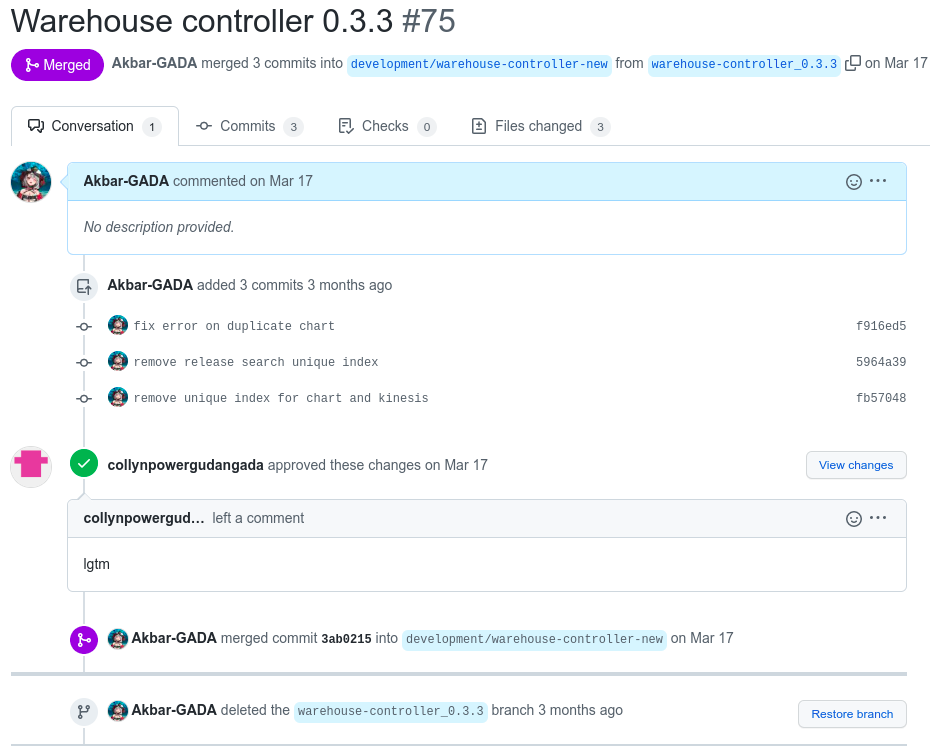
\includegraphics[width=1\textwidth]{pics/wc-lgtm.png}
	\caption{Pemilik repositori memberikan lampu hijau untuk melakukan \textit{merge} ke repositori Data Warehouse GudangAda}
	\label{fig:wcLGTM}
\end{figure}

\subsection{Membuat dan Mengirimkan Docker \textit{Image} ke Repositori GudangAda}
\label{sec:uploadDocker}

Setelah aplikasi disetujui oleh pemilik repositori, aplikasi dapat di kemas ke dalam sebuah \textit{image} dan dikirimkan ke repositori GudangAda. Pembuatan \textit{image} dilakukan dengan menjalankan perintah \code{docker build -t IMAGE\_NAME:TAG .} pada direktori aplikasi. Hasil dari perintah tersebut dapat dilihat pada gambar \ref{fig:dockerBuild}

\begin{figure}
	\centering
	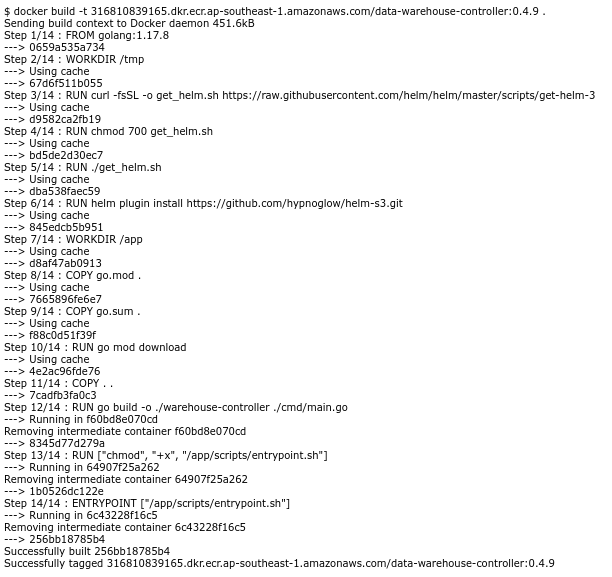
\includegraphics[width=1\textwidth]{pics/image-build.png}
	\caption{Membuat Docker \textit{image}}
	\label{fig:dockerBuild}
\end{figure}

Setelah \textit{image} aplikasi berhasil dibuat, \textit{image} tersebut harus dikirimkan ke repositori GudangAda. Hal ini dilakukan agar Terraform dapat memakai \textit{image} yang telah dibuat. Pengiriman \textit{image} dilakukan dengan perintah \code{docker push IMAGE\_NAME:TAG}. Hasil dari perintah tersebut dapat dilihat pada gambar \ref{fig:dockerPush}

\begin{figure}
	\centering
	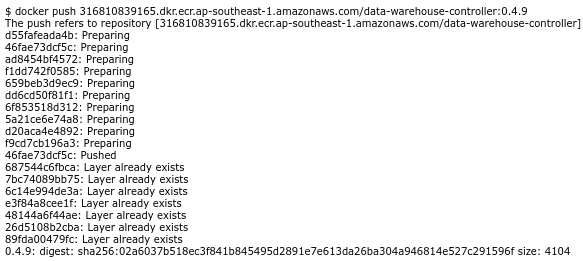
\includegraphics[width=1\textwidth]{pics/image-push.png}
	\caption{Mengirimkan Docker \textit{image} ke repositori GudangAda}
	\label{fig:dockerPush}
\end{figure}

\subsection{Data Helm Chart}
\label{sec:mergeHelmChart}

GudangAda menggunakan Amazon S3 sebagai repositori Helm Chart. Repositori tersebut tersinkronsasi dengan repositori GitHub \code{data-helm-chart}. Semua kode yang berada pada branch master akan ditambahkan ke Amazon S3. Oleh karena itu, proses untuk menambahkan Helm Chart ke repositori Amazon S3 adalah membuat \textit{merge request} untuk diperiksa oleh pemilik repositori. Setelah pemilik repositori menyetujui Helm Chart yang ditulis, Helm Chart tersebut dapat digabungkan dengan Helm Chart lain pada repositori GitHub. 

\begin{figure}
	\centering
	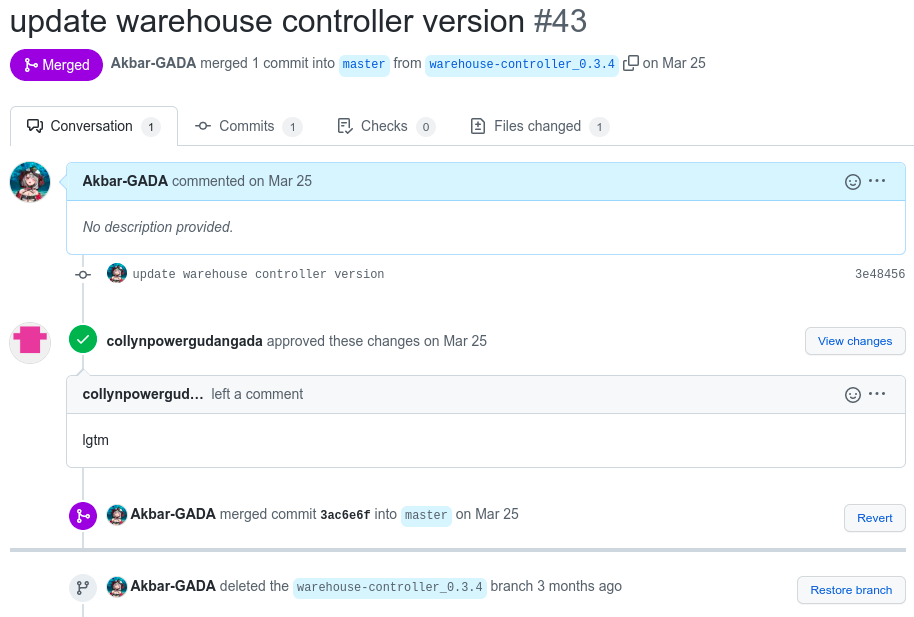
\includegraphics[width=0.75\textwidth]{pics/chart-lgtm.png}
	\caption{Pemilik repositori memberikan lampu hijau untuk melakukan \textit{merge} ke repositori Data Helm Chart pada GitHub GudangAda}
	\label{fig:wcLGTMTF}
\end{figure}

\subsection{Data IAAC}
\label{sec:mergeTerraform}
Proses \textit{deployment} menggunakan Terraform dilakukan dengan membuat \textit{request merge} ke \textit{repository} data IAAC. Setelah pemilik repositori melakukan \textit{review} terhadap perubahan yang akan dilakukan. Proses \textit{deployment} dapat dimulai.

\begin{figure}
	\centering
	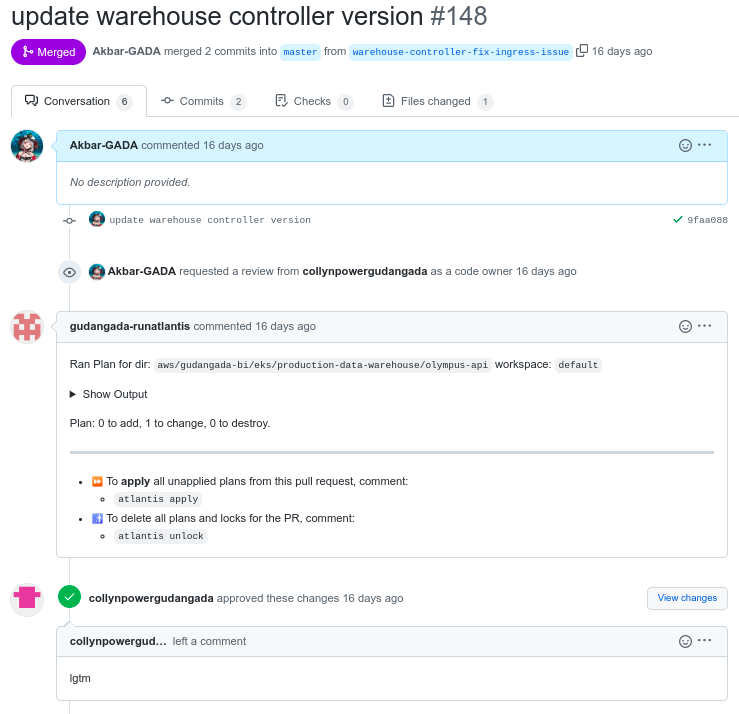
\includegraphics[width=0.75\textwidth]{pics/github-lgtm.png}
	\caption{Pemilik repositori memberikan lampu hijau untuk memulai proses deployment}
	\label{fig:githubLGTM}
\end{figure}

Proses \textit{deployment} dilakukan dengan melakukan \code{atlantis plan}, perintah ini bertujuan untuk menghitung semua kebutuhan \textit{deployment}, \code{atlantis plan} dilakukan secara otomatis saat \textit{merge request} dibuat. Setelah perintah \code{atlantis plan} selesai, akan dikirimkan perintah \code{atlantis apply} untuk menjalankan semua kebutuhan \textit{deployment} yang didapat dari \code{atlantis plan}. Setelah perintah \code{atlantis apply} selesai, kode sudah berhasil di deploy dan kode dapat di \textit{merge} ke repositori GudangAda.

\begin{figure}
	\centering
	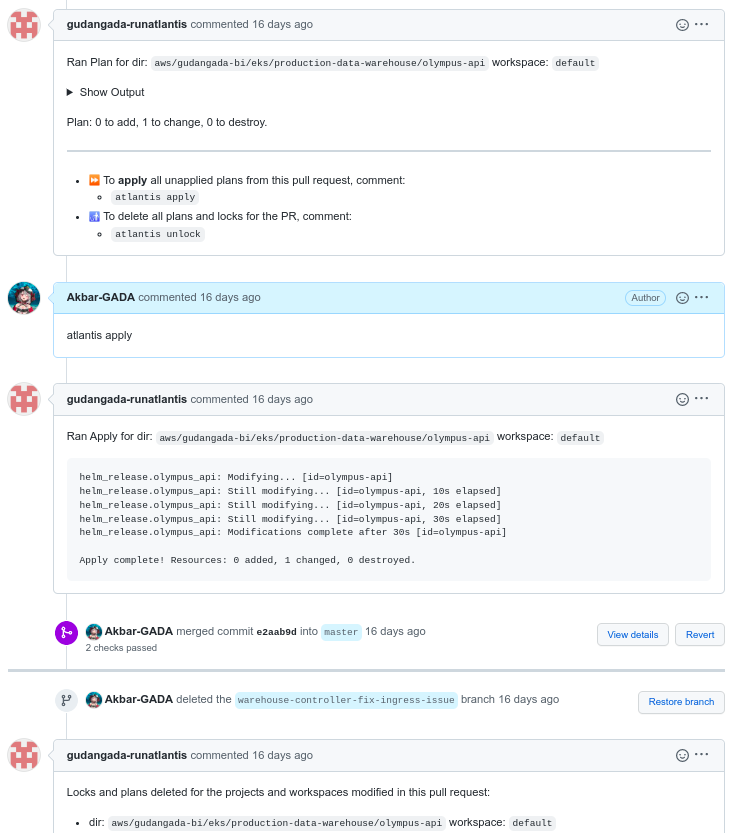
\includegraphics[width=0.75\textwidth]{pics/github-merge.png}
	\caption{Proses deployment menggunakan Terraform}
	\label{fig:githubMerge}
\end{figure}